% 
% Annual Cognitive Science Conference
% Sample LaTeX Paper -- Proceedings Format
% 

% Original : Ashwin Ram (ashwin@cc.gatech.edu)       04/01/1994
% Modified : Johanna Moore (jmoore@cs.pitt.edu)      03/17/1995
% Modified : David Noelle (noelle@ucsd.edu)          03/15/1996
% Modified : Pat Langley (langley@cs.stanford.edu)   01/26/1997
% Latex2e corrections by Ramin Charles Nakisa        01/28/1997 
% Modified : Tina Eliassi-Rad (eliassi@cs.wisc.edu)  01/31/1998
% Modified : Trisha Yannuzzi (trisha@ircs.upenn.edu) 12/28/1999 (in process)
% Modified : Mary Ellen Foster (M.E.Foster@ed.ac.uk) 12/11/2000
% Modified : Ken Forbus                              01/23/2004
% Modified : Eli M. Silk (esilk@pitt.edu)            05/24/2005
% Modified: Niels Taatgen (taatgen@cmu.edu)  10/24/2006

%% Change ``a4paper'' in the following line to ``letterpaper'' if you are
%% producing a letter-format document.








%% --------- Short APA CITE Helpfile  --------- %%
%% 	Command									Result
%%	\cite<e.g.,>[p.~11]{Jone01,Ross87}				(e.g., Jones, 2001; Ross, 1987, p. 11)
%%	\citeA<e.g.,>[p.~11]{Jone01,Ross87}				e.g., Jones (2001); Ross (1987, p. 11)
%%	\citeauthor<e.g.,>[p.~11]{Jone01,Ross87}			e.g., Jones; Ross, p. 11
%%	\citeyear<e.g.,>[p.~11]{Jone01,Ross87}			(e.g., 2001; 1987, p. 11)
%%	\citeyearNP<e.g.,>[p.~11]{Jone01,Ross87}		e.g., 2001; 1987, p. 11
%%	\citeNP<e.g.,>[p.~11]{Jone01,Ross87}			e.g., Jones, 2001; Ross, 1987, p. 11
%%


\documentclass[10pt,letterpaper]{article}

\usepackage{cogsci}
\usepackage{pslatex}
\usepackage{apacite}
\usepackage{graphicx}
\usepackage{color}
\usepackage{amsmath}
\usepackage{multirow}
\usepackage{amssymb}
%\usepackage{url}
%\usepackage{hyperref}


 
\definecolor{Red}{RGB}{255,0,0}
\newcommand{\red}[1]{\textcolor{Red}{#1}}  


%\title{ Lay theories of emotion in explaining behavior }
\title{ Where is the Love (in folk psychology)? \\ Emotions in lay explanations of behavior }
 
\author{{\large \bf Desmond C. Ong (dco@stanford.edu)} \\
{\large \bf Jamil Zaki (jzaki@stanford.edu))} \\
{\large \bf Noah Goodman (ngoodman@stanford.edu)} \\
  Department of Psychology, Stanford University, Stanford CA, USA 
}

\begin{document}

\maketitle

\begin{abstract}
Abstract \\
\\
\\
\\
\\
\\


\textbf{Keywords:} 
Keywords
\end{abstract}

% Outline of paper

% More free-form
% Expt 1a) Emotions --> Actions
% Expt 1b) Generate cause of Actions. Coded into emotions, beliefs, situational factors, etc.

% More hypothesis driven
% Expt 2a) Actions / Expressions / Behavior, generate causes: Beliefs, Desire, Emotion, Situation factor
% Expt 2b) From 2a, for all actions/expressions/behavior, pick top b,d,e,s. Find endorsement rates of posterior using sliders.




% Start with a quote from the BARD. Maybe even Othello


\begin{quote}
\textit{``... men in rage strike those that wish them best"} 
--- Iago, in Shakespeare's \textit{Othello}, perhaps subtly presaging the (Iago-instigated) murder of Desdemona by Othello's hands. (Act 2, Scene 3, line 205) \red{to fix: proper citation}
\end{quote}

%2.3.205 % act 2, scene 3, line 205


We have a rich intuitive understanding of other people and their emotions \cite{Ong2015AffCog}. In his plays, the Bard of Avon makes masterful use of the lay person's understanding of emotion: in \textit{Othello}, the audience is privy to Iago's deliberate manipulation of Othello's jealousy and rage, and can effortlessly predict Othello's murder of Desdemona before it happens. Consider the counterfactual scenario: would Othello still have killed Desdemona had he not been feeling those emotions? This seems unlikely; intuitively, emotions played a key, irreplaceable role in Othello's decision making process.

We naturally extend this type of powerful reasoning to explain the behavior of others, both fictional and nonfictional. This process of applying knowledge to reason about the mental states and behavior of others is often called folk psychology, or lay psychology \cite<e.g., >{Heider1958, Malle2011}. Many modern theories posit a ``belief-desire psychology" \cite<e.g., >{Bartsch1995, Gopnik1997, Malle1999, Malle2011, Searle2001}, in which an agent has a set of goals (often termed \textbf{desires}), and a set of ideas or beliefs about the world on how to achieve those goals (often termed \textbf{beliefs}). The agent then forms an intention to act upon his beliefs to achieve his desires, resulting in \textbf{intentional action}. The tendency to attribute such \textit{intentionality} to agents forms what \citeA{Dennett1989} famously termed an ``intentional stance", is pervasive in lay psychology, and arises as early as 12 months of age \cite{Gergely1995}. When laypeople are asked to explain an agent's behavior, they often appeal to the beliefs and desires of the agent that spur their actions: ``Sue went to the store at 3pm, because (1) she wanted a drink, and (2) she thinks that the store sells alcohol". Laypeople also offer as explanations upstream events that resulted in a belief or desire (\citeNP{Malle1999}'s \textit{Causal History of Reasons}): ``Sue had a bad argument (which caused her to want a drink)", or ``Sue goes to the store everyday (so she knows it sells alcohol)". A fourth class of reasons that laypeople give are \textbf{Enabling Factors}: events that facilitated the feasibility of the intentional action, but did not instigate it: ``Sue got out of work early (which allowed her to go get a drink at 3pm)". Finally, these theories also account for the case of non intentionality. \textbf{Unintentional behavior} are often described as a result of \textbf{situational factors} via physical causality (or \textit{impersonal causality}; \citeNP{Heider1958}): ``Sue slipped and fell because there was ice on the floor (not because she intended to)". This taxonomy has proven incredibly fruitful and productive in explaining how lay people explain behavior.

Sadly, these models are often emotionless\footnote{pun intended} and relegate emotions to the bin of other, situational causes. For example, in these models, feeling sad makes one cry, an ``unintentional" behavior that is out of the control of the agent. There is an implicit assumption that emotion-driven behavior is unintentional, or sometimes, just plain irrational. Importantly, these models do not account for how lay people use emotions in causal explanations, such as how an agent's emotional state might influence the formation of intentions. It is worth noting that many scientific theories of emotion include behavior as a crucial part of their definitions of emotion. On one hand, emotions cause characteristic ``automatic" behavioral responses like facial expressions and vocalizations \cite<e.g.,  >{Ekman1992}: these expressions are also influenced by cultural display rules \cite<e.g., >{Matsumoto1990} and other top-down cognitive processes. On the other hand, emotions also bias organisms towards certain types of actions via \textit{action tendencies} \cite{Frijda1989, Fontaine2007} or approach/avoid motivations \cite<e.g., >{Carver2004}. For example, being in a state of happiness predisposes one towards helping others \cite{Isen1972} and risk-taking \cite{Isen1983}. Lay people do have this intuition that emotions influence intentional actions (``he replied my email; the boss must be in a good mood today"). Returning to the example of Othello, we argue that even his beliefs (that Desdemona cheated on him) and his desires (perhaps, to punish her) alone, without any rage, would not have led him to murder his wife. 

%and this has made its way into legal attributions of guilt and responsibility, as in crimes of passion like Othello's. \textit{\red{I need to work on this last line, and crime might not be the best way to end here...}}

% TODO: finish this part

In this paper we provide some preliminary explorations of how emotions are incorporated into lay belief-desire psychology, and specifically, how emotions are used or judged as explanations of intentional actions. First, we begin by laying out three possible models: each provides distinct, testable predictions that we explore via experiments with lay participants. In Study 1, we study the types of actions that laypeople think emotions cause, and show that the top emotion-caused actions are judged to have been caused by emotions only about half the time. In Study 2, we show that laypeople are willing to endorse emotions as causes of intentional actions. We also find that people are willing to endorse beliefs and desires as likely causes of emotional expressions (e.g., smiling), which has previously been treated as unintentional behavior in previous lay theories. This paper provides but a first step in exploring how emotions are used by laypeople in explaining behavior, and we end by discussing future directions that are inspired by this research.

%\red{[TODO: finish this part with results]}




%moral evaluations (Knobe, 2003)





%One hypothesis is that in our lay theories of behavior, there are two distinct processes that result in two types of behavioral responses (see Fig. \ref{ModelsOfBehaviorFig}a). The first of these processes is a rational decision making process in which an agent has a set of goals (``desires"), and a set of ideas on how to achieve those goals (often termed ``beliefs"). The agent then forms an intention to act upon his beliefs to achieve his desires, resulting in (intentional) action, as part of a ``belief-desire psychology" \cite{Dennett1989, Gopnik1997, Heider1958, Malle2011, Searle2001}. 


%The second process, by contrast, relies on mere causality or ``impersonal causality" \cite{Heider1958}, and results in a second type of behavioral response. 


\section{Three possible theories of behavior}


\begin{figure}[htb!]
\begin{center}
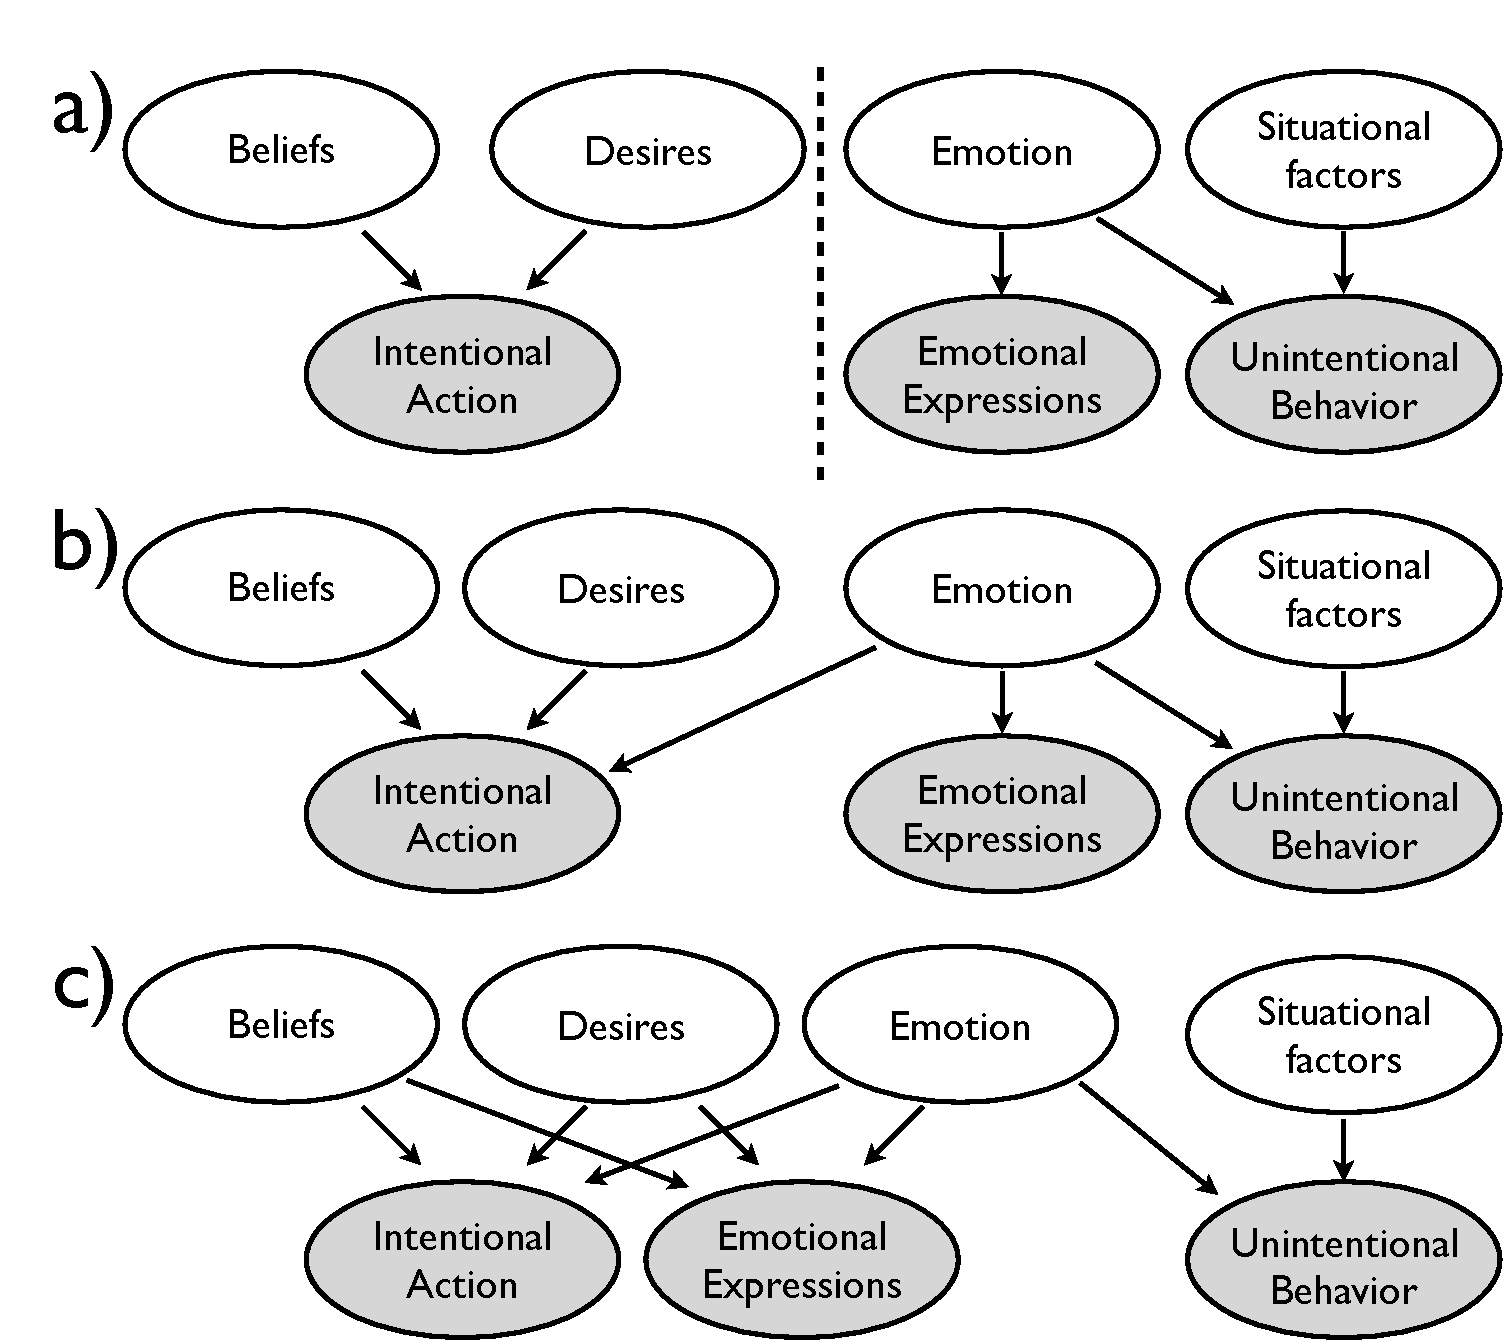
\includegraphics[width=1\columnwidth]{images/model1.pdf} 
\end{center}
\caption{ Possible lay theories of behavior. (a) There are two distinct types of behavioral responses; the rational decision-making process that goes from beliefs and desires to intentional action, and unintentional behavior and emotional expressions that are caused by situational factors and emotions. The latter process is governed by simple causality, without the need for an agent's intentionality. (b) Emotions do factor into the intentional decision making process, but there still exists emotional expressions and other unintentional behavior that are unaffected by beliefs and desires. (c) There is no sharp distinction between intentional action and emotional expressions in that both are affected by beliefs, desires and emotions.  }
\label{ModelsOfBehaviorFig}
\end{figure}


Let us begin by writing down several models which provide more concrete hypotheses. The first model, built off the literature on belief-desire psychology, posits that lay people distinguish two distinct processes that result in two types of behavioral responses (see Fig. \ref{ModelsOfBehaviorFig}a). The first of these two processes assumes that agents have \textbf{Beliefs} and \textbf{Desires}, which interact, giving rise to \textbf{Intentional Actions}. The second process, by contrast, relies on mere causality, and results in a second type of behavioral response. Here, we specifically distinguish between two types of ``other causes", \textbf{Emotions} (e.g., sadness) and \textbf{Situational Factors} (e.g., the ground is icy), and two types of behavior: \textbf{Emotional Expressions} (e.g., crying, laughing), and \textbf{Unintentional Behavior} (e.g., slipping on ice, snoring). Previous theories have subsumed Emotional Expressions into Unintentional Behavior: here, we assume that the former is only caused by emotions, whereas the latter could be caused by situational factors and possibly, emotions (this is to allow emotions to explain unintended ``irrational" behavior). Notably, in these theories of folk psychology, there is no place for emotions in the ``rational" decision making process that humans reason with when explaining the actions of others.
% Probably can say a bit more in the above paragraph when I read those papers.


A second model accounts for the hypothesis that emotions do play an important role in the formation and execution of intentional action. Figure \ref{ModelsOfBehaviorFig}b posits a lay theory in which emotions are factored into the intentional decision making process. This approach been incorporated into psychological \cite<e.g., >{Schwarz2000emotion}, economic \cite<e.g., >{Loewenstein2003affect}, and philosophical \cite<e.g., >{Zhu2002emotion} theories of behavior, but it is unclear how a theory of folk psychology incorporates emotions into the lay model of decision making \cite{Ong2015AffCog}. Here, we simply assume that emotions somehow influences the intentional decision making process---in the Discussion, we return to how exactly this might occur.

A third possibility that we must also consider is that the distinction between intentional action and emotional expressions in the lay theory is needlessly strong (Fig. \ref{ModelsOfBehaviorFig}c), and that emotions, as well as beliefs and desires, impact both an agent's intentional actions and emotional expressions. Indeed, emotional display rules \cite<e.g., >{Matsumoto1990} and deceptive strategies \cite<e.g., >{Depaulo2003} do impact an agent's displayed emotional expressions, and might very well be an important factor in lay explanations of behavior. %However, we (as have many theorists before us) reject the notion that all instances of emotional expressions are intentional, and hence should not be a subset of intentional action.



In order to test this, we used a free-response paradigm to have lay people generate actions from emotions (Study 1a), and causes of these actions (Study 1b), to show that emotion-caused actions are judged likely to be caused by other, non-emotional causes. We then tested the three models more rigorously by elicited judgments of explanations of intentional actions, emotional expressions, and unintentional behavior (Study 2).


%%%%

\section{Study 1a: Emotions to Actions}

	In Study 1a, we elicited participants' free-response nominations of emotion-caused actions. We then obtained judgments of the counterfactual likelihood (i.e., how likely were their nominated actions, if the agent had not felt the emotion). This allowed us to test lay intuitions of whether the given emotions are both sufficient (via the nomination) and necessary (via the counterfactual judgments) for the actions. Samples of all studies reported in this paper are available here\footnote{https://github.com/desmond-ong/shakespeare/Cogsci}.

% Expt 1a) Emotions --> Actions
% Expt 1b) Generate cause of Actions. Coded into emotions, beliefs, situational factors, etc.

\subsubsection{Participants and Procedures.} 
We recruited 100 participants (99\% had English as their native language) through Amazon's Mechanical Turk (AMT). Participants saw statements of the form ``Bob \underline{\hspace{3em}} because he was [\textbf{emotion}]", and were asked to give sentence completions. The presented \textbf{emotion} was one of: \{happy, calm, anger, sad, surprised\}\footnote{We chose a high-arousal positive valence (``happy"), a low-arousal positive valence (``calm"), a high-arousal negative valence (``anger"), a low-arousal negative valence (``sad"), and a high-arousal neutral valence (``surprised") emotion.}. On each page, participants saw only one emotion, and gave 5 different completions (for a total of 25 completions). The emotions were presented in a random order; names were randomized on every sentence.

After participants had given completions to all 5 emotions, they were then presented their answers, and asked to rate the likelihood of the counterfactual: ``You wrote that `\textit{Bob [cried] because he was [sad]}'. If Bob was not feeling [sad], would he still have [cried]?" Participants gave responses on a 7 point Likert scale from ``Very Unlikely" to ``Very Likely". 




\subsubsection{Results.} 
We grouped similar free-responses together (e.g., ``smiled", ``smiled widely", and ``beamed"), and present the top 5 responses for each emotion in Table \ref{Study1aResultsTable}. Note that, as expected, the majority of these modal responses would easily be judged to be \textit{emotional expressions}: some notable exceptions are ``killed himself"\footnote{It is unfortunate that this is one of the modal lay responses for what an agent will do when he is sad...}, ``punched the wall", ``slept", and ``sat down".


\begin{table}
\scalebox{0.80}{
\begin{tabular}{l l l l l}
\textbf{Happy} & \textbf{Calm} & \textbf{Sad} & \textbf{Anger} & \textbf{Surprised} \\
%\hline
smiled: 63 & relaxed: 50 & cried: 97 & ``hit X": 56 & jumped: 65 \\
laughed: 51 & slept: 46 & frowned: 17 & yelled: 54 & laughed: 41 \\
\multirow{2}{*}{jumped: 42} & \multirow{2}{*}{sat down: 32} & killed & \multirow{2}{*}{screamed: 21} & \multirow{2}{*}{screamed: 30} \\
& & himself: 13 & & \\
danced: 22 & smiled: 26 & slept: 13 & cried: 15 & yelled: 25 \\
cried: 21 & sighed: 10 & yelled: 13 & cursed: 12 & smiled: 23 \\
\end{tabular}
}
\caption{ Action nominations from emotions (Study 1a). Top 5 responses for each emotion, with nomination counts in parentheses. The most common responses for anger were variants of ``hit X", where X is an object or person (of these, the modal response was: ``punched the wall"). }
\label{Study1aResultsTable}
\end{table}

%\multirow{2}{*}{text}

The nomination portion allowed us to test sufficiency: if a participant nominated an action $a$ when given emotion $e$, then the emotion $e$ is sufficient to have caused that action $a$. We turn next to the counterfactual rating task, to investigate necessity. We hypothesized that the more often a particular action $a$ is nominated for emotion $e$ across all participants, the more \textit{necessary} is emotion $e$ for action $a$ to occur. Hence, we should expect that these commonly nominated actions $a$ would be less likely to happen in the absence of emotion $e$. In order to test this, we regressed participants' counterfactual likelihood ratings (i.e., how likely is the action to occur if the emotion was absent, $P(A | \neg E)$) against the frequency of that action being nominated across the sample, with random intercepts by participant and emotion. We find that, across all emotions, the more frequently an action is nominated, the less likely participants rate it to occur in the absence of the emotion $(b = -0.0084, 95\% \text{ CI}: [-0.0108, -0.0060], t=-6.82, p<0.001$; See Fig. \ref{Study1aResultsFig}). Thus, the modal nominated actions are judged less likely to occur in the absence of the corresponding emotions, and thus, in participants' lay theories, the corresponding emotions are more necessary for these actions to occur: we shall use this result in Study 1b.



\begin{figure}[htb!]
\begin{center}
	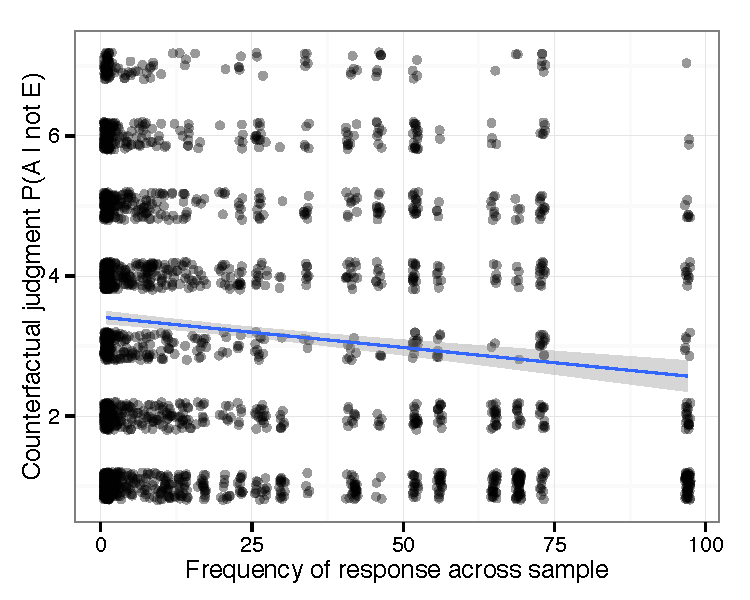
\includegraphics[width=1\columnwidth]{images/study1a_results.pdf}
\end{center}
\caption{ Study 1a Results. Individual counterfactual likelihood ratings ($P(A | \neg E)$) against frequency of an action's nomination across the sample. Data points are transparent and jittered for clarity. }
\label{Study1aResultsFig}
\end{figure}


\section{Study 1b: Causes of Actions}

	In Study 1b, we recruited a separate group of participants to give explanations for the modal actions nominated from Study 1a. Lay participants from Study 1a judged emotions to be both sufficient and necessary for these modal actions to occur: hence, if Model 1 (Fig. \ref{ModelsOfBehaviorFig}a) were correct, in Study 1b, we should only expect explanations due to emotions (and perhaps, situational factors).


\subsubsection{Participants and Procedures.} 
In a similar manner to Study 1a, we recruited 100 participants through AMT (98\% had English as their native language). This time, participants saw statements of the form ``Bob [\textbf{action}] because \underline{\hspace{3em}}", and were asked to complete the sentence. The presented \textbf{action} was one of fifteen possible actions drawn from the most popular nominations from Study 1a (i.e., the 15 unique actions in Table \ref{Study1aResultsTable}, with ``punched the wall" used in place of ``hit X"). Participants gave 1 completion per action and saw the actions in a random order.

\subsubsection{Results.} 
The free-response completions were coded into one of five categories: (a) ``\textbf{Emotion}" (if there was a mention of an emotion word), (b) ``\textbf{Cause of Emotion}" (if there was a mention of an event that would cause an emotion, e.g., ``his dog died"), (c) ``\textbf{Physical state}" (if the explanation referenced a physical state like tiredness or pain), (d) ``\textbf{Mental state}" (if the explanation referenced a desire or a belief); (e) ``\textbf{Situation}" (for enabling and other situational factors). 

The distribution of coded free-responses is given in Figure \ref{Study1bResultsFig}. If the actions generated from Study 1a were characteristic of those emotions, and if they could only have been caused by emotions (i.e., Fig. \ref{ModelsOfBehaviorFig}a), then we should expect the vast majority of the explanations to be due to emotions, or to upstream causes of emotions\footnote{``Because he is sad" is a somewhat unsatisfying explanation to ``why is he crying?" in conversation, and often begs the question ``well, so what made him sad?". People often give Causes of Emotion as explanations for (obvious) emotions, and so we decided to code specifically for these.}. However, we see that in fact, only 40.7\% of explanations appeal to an Emotion, and 51.7\% appeal to an Emotion or to a Cause of an Emotion. There are many other references to Physical states (e.g. physical pain as a cause for ``cursing" or ``yelling"; fatigue as a cause of ``sat down" or ``slept"), or to Mental states (e.g. a belief or a desire). Thus, it seems very likely that lay people's judgments of emotion-caused actions are not, in fact, predominantly caused only by emotions, which might support a more parsimonious model, as in Figure \ref{ModelsOfBehaviorFig}c. We test this model more precisely in Study 2.

\begin{figure}[htb!]
\begin{center}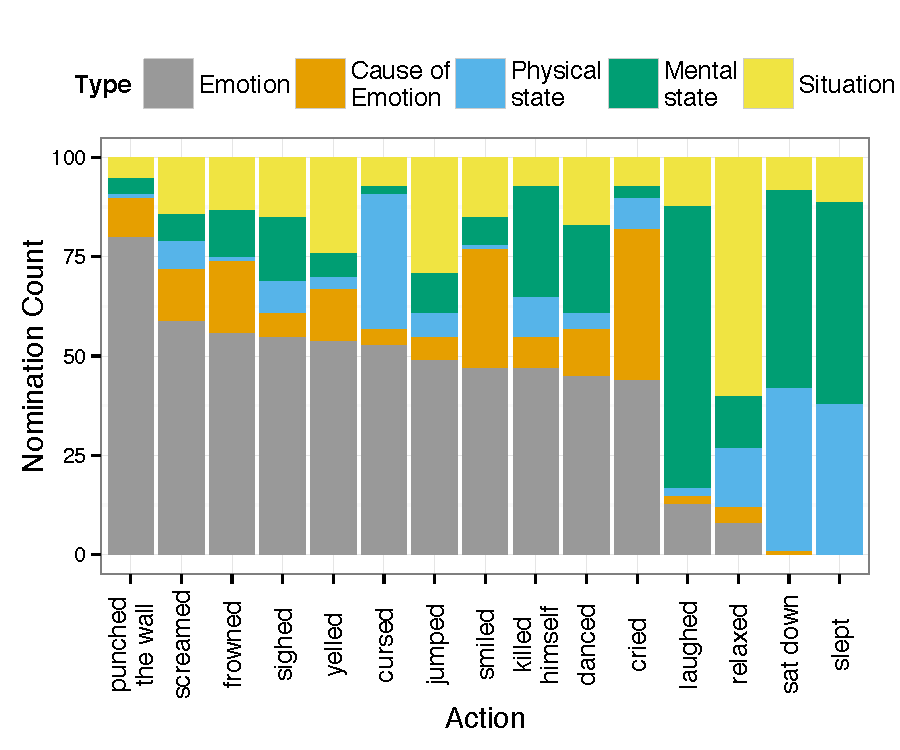
\includegraphics[width=1\columnwidth]{images/study1b_codePlot.pdf}\end{center}
\caption{ Results of Study 1b. We plot the number of nominations that fall into each explanation type for each action. }
\label{Study1bResultsFig}
\end{figure}


\section{Study 2: Rating explanations for actions}


%In Study 1a/b, we examined participants' judgments of actions from several emotions, and we did not impose any formal structure on the type of actions that people generated (e.g., whether they were intentional actions or emotional expressions). 
In Study 2, we sought to test Figure \ref{ModelsOfBehaviorFig}c in more precisely. First, we chose a set of actions (that span Intentional Actions, Emotional Expressions, and Unintentional Behavior), and asked participants to rate how likely it was that each action was caused by Belief, Desire, Emotion, or Situational Factor explanations. Importantly, we had two aims in this study: (1) to demonstrate that people judge emotions as suitable explanations for intentional behavior (the Emotion to Intentional Action arrow in Fig. \ref{ModelsOfBehaviorFig}b and \ref{ModelsOfBehaviorFig}c), and (2) to a lesser extent, people judge beliefs and desires as suitable explanations for emotional expressions (Fig. \ref{ModelsOfBehaviorFig}c). Although the three models do not differentiate between the causes of Unintentional Behavior, we included Unintentional Behavior and Situational Factors in order to test baseline predictions that all three models should make, hence verifying the validity of our paradigm.

\begin{figure*}[htb!]
\begin{center}
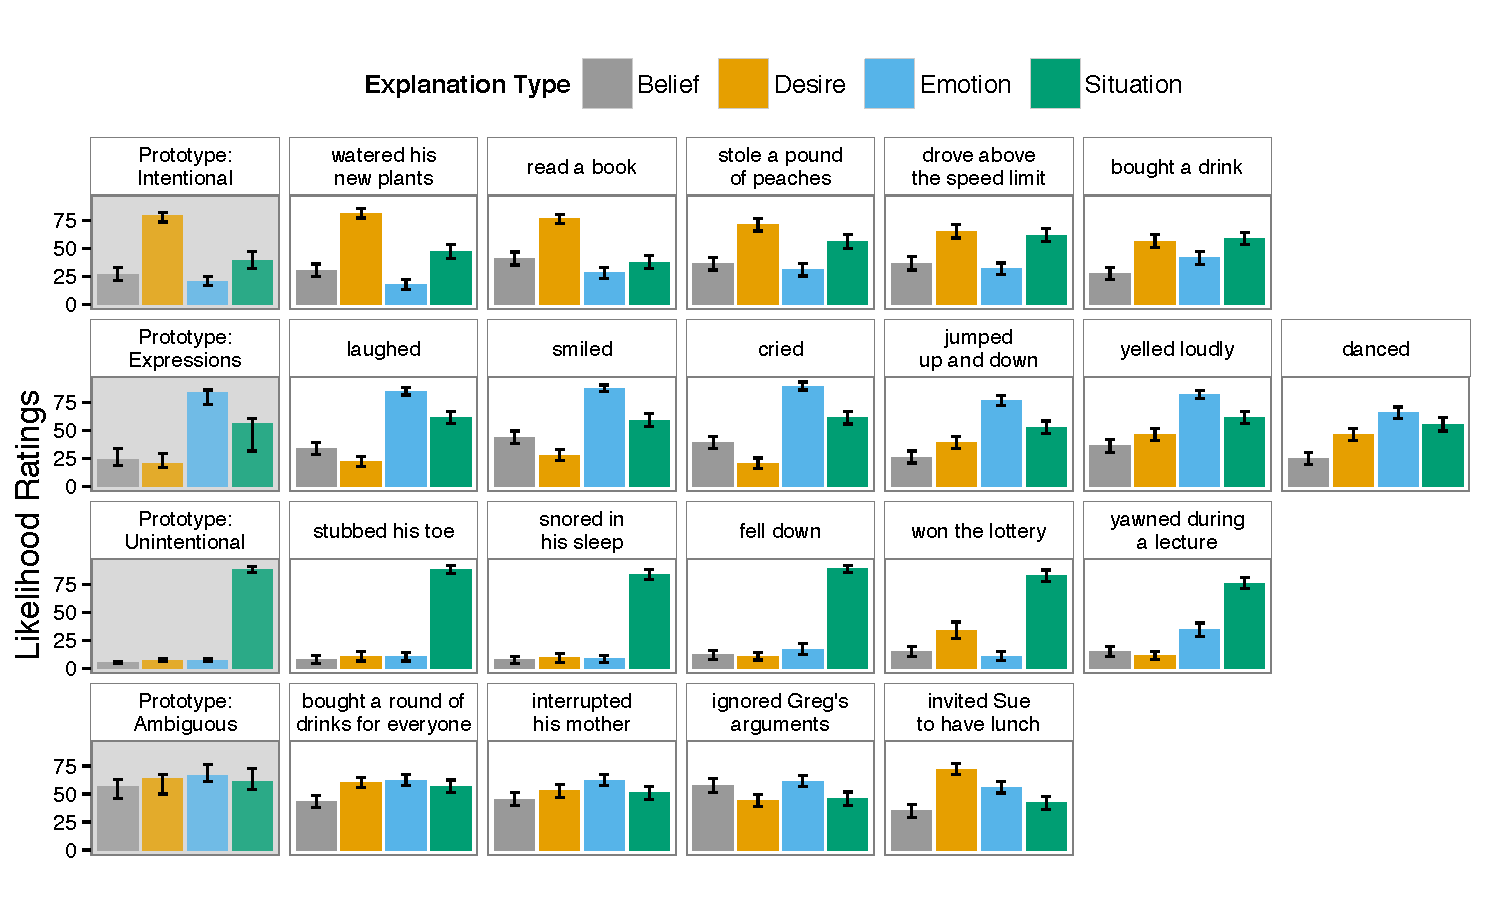
\includegraphics[width=1\linewidth]{images/study2Results.pdf}\end{center}
\caption{ Results of Study 2. Mean ratings of how likely each explanation type was to have caused the action. The left most column, shaded in grey, illustrate our a priori predictions (discussed in detail in the text). Error bars on empirical data indicate 95\% confidence intervals. }
\label{Study2ResultsFig}
\end{figure*}


\subsubsection{Stimuli Selection.} We selected a set of 20 actions, comprising a mix of 6 intentional actions, 6 emotional expressions, 5 unintentional behaviors, and 3 ambiguous behaviors. Of the 6 intentional actions, we chose 3 of them (``stole a pound of peaches"; ``invited Sue to have lunch"; and ``watered his new plants") from \citeA{Malle1999}'s study as they were previously rated as very highly intentional. We chose the 6 emotional expressions from the modal responses of Study 1a (i.e., from Table \ref{Study1aResultsTable}). We chose two unintentional behaviors (``yawned during a lecture", ``won the lottery") from \citeA{Malle1999}'s list, as they were rated as being low on intentionality. Finally, we chose 3 ``ambiguous" behaviors (``drove above the speed limit"; ``ignored Greg's arguments"; ``interrupted his mother"), all from \citeA{Malle1999}'s study, which were rated by some of their participants as being intentional, and others as being unintentional.

\subsubsection{Participants and Procedures.} 
We recruited 100 participants through AMT (98\% had English as their native language; 1\% did not report).
First, participants learnt about different types of explanations, with examples of each. We chose to use more lay terms for some of the explanation types (1) \textbf{Thoughts}, which are thoughts or beliefs that make people behave so (``Bob moved to Iowa because he \textbf{thinks} people are nice there"); (2) \textbf{Emotions}, (``Bob ran away because he was \textbf{feeling} scared"); (3) \textbf{Aims}, and people behave to achieve a certain aim (``Bob kicked the ball because he \textbf{wanted to} win the game"); and (4) \textbf{Situational Causes}, whereby the situation makes them behave so (``Bob shivered because it was cold outside").

Next, participants saw statements of the form ``Bob [\textbf{action}] because ...", followed by descriptions of four explanation types: (``... he was motivated by some thoughts or beliefs about the way the world is"; ``... he felt some emotions"; ``... he wanted to achieve some aims of his"; ``of some situational causes"). They then used continuous, 100 point sliders to rate how likely it was that the behavior was caused by each type of cause, from ``Not at all likely" to ``Extremely likely". Participants completed the 20 actions in a random order.


\subsubsection{Results.} 
Participants' mean ratings for each action, along with our a priori predictions, are shown in Figure. \ref{Study2ResultsFig}. First, let us outline our predictions, in the left most column. Importantly, if the model in Figure \ref{ModelsOfBehaviorFig}c was correct, we might hypothesize that: 
\begin{enumerate}
\item For Intentional Actions (1st row), \textbf{B}eliefs and \textbf{D}esires will be rated as the most likely causes, and \textbf{E}motion ratings will be in the middle. ($B,D>E>S$)
\item For Emotional Expressions (2nd row), \textbf{E}motion explanations will be rated as the most likely, while ratings of \textbf{B}eliefs and \textbf{D}esires will be endorsed to a small extent. ($E \gg B,D>S$)
\item For Unintentional Behavior (3rd row), we should see high ratings for \textbf{S}ituational Factor causes, and low endorsements for other types of causes. ($S\gg B,D,E \sim 0$)
\item Ambiguous Behavior (4th row) were judged by previous participants \cite{Malle1999} as being intentional and others as being unintentional. Thus, we hypothesized to see a mix of responses for Intentional and Unintentional. Averaging across many participants, this should result in mediocre ratings for all four types of causes. ($B=D=E=S > 0$)
\end{enumerate}

By and large, participants' mean ratings across all the actions matched our predictions.

\red{What stats should I do?}



\section{Discussion}

Using sentence completions to study intuitive theories

How do emotions affect intentional action?
Influence beliefs
Influence desires
Influence other than via beliefs/desires.
All these are ripe for future work!


\section{Acknowledgments}

This work was supported in part by an A*STAR National Science Scholarship to DCO and by \red{[TODO:] XXX to NDG}.


\bibliographystyle{apacite}

\setlength{\bibleftmargin}{.125in}
\setlength{\bibindent}{-\bibleftmargin}

\bibliography{shakespeare_cogsci}




%In Study 1a/b, we examined participants' judgments of actions from several emotions, and we did not impose any formal structure on the type of actions that people generated (e.g., whether they were intentional actions or emotional expressions). In Study 2, we sought to test Figure \ref{ModelsOfBehaviorFig}c in a more hypothesis driven manner. First, we chose a set of actions (that span Intentional Actions, Emotional Expressions, and Unintentional Behavior), and specifically elicited Belief, Desire, Emotion, and Situational Factor explanations for these actions. We then collected, on a separate sample, ratings on the modal responses to each of these explanations. Under Figure \ref{ModelsOfBehaviorFig}c, we might hypothesize that (1) Beliefs and Desires will be rated highest as causes for Intentional Actions, although Emotion ratings will also be high, (2) Emotion ratings will be highest for Emotional Expressions, and ratings of Beliefs and Desires will also be high, and (3) For Unintentional Behavior, we should see high ratings for Situational Factor causes, and low ratings on other types of causes.
%
%\subsection{Generating lay explanations.} 
%To generate plausible lay explanations of behavior, we recruited 100 participants through AMT (97\% had English as their native language; 1\% did not report). Participants read about four different types of explanations for behavior: \textbf{thoughts} (i.e., beliefs about the state of the world), \textbf{emotions}, \textbf{aims} (i.e., desires), and \textbf{situational causes}. They read simple lay definitions of these four types of causes, and read examples of each (e.g. ``Bob moved to Iowa because he thinks people are nice there"). Then, participants saw statements and gave four different explanations for each statement, e.g. ``Bob [\textbf{action}] because he thought \underline{\hspace{3em}} (please give a thought)". Thus, whereas in Study 1b, we elicited only one explanation per action, here in Study 2a we prompted participants for 4 possible explanations per actions. We chose a set of 10 actions that consisted of a mix of 4 intentional actions (taken from \citeNP{Malle1999}), 3 unintentional actions (e.g. ``snored in his sleep"), and 3 emotional displays (from Study 1a: ``smiled", ``cried", and ``yelled"). The modal responses served as stimuli for the rating task, below.

% intentional actions after Malle 1999
%watered his new plants
%invited Sue to have lunch
%stole a pound of peaches
% drove above the speed limit

% smiled
% cried
% yelled

% slipped and fell
% snored in his sleep
% stubbed his toe

%\subsection{Rating Task}
%For the rating task, we recruited a separate group of 100 participants through AMT (X\% had English as their native language).


\end{document}
